\section{Observation and Calculations}

\subsection{Magnetoresistance}

\subsubsection*{Spatial Distribution of the Magnetic Field}

In the first part of the experiment, we set the pole piece distance of the electromagnet to approximately 19 mm, ensuring sufficient space for the magnetoresistance probe. We verified that the electromagnet produced a magnetic field by supplying current
and measuring it using a Hall sensor. Due to the geometry of the setup, the magnetic field might not be constant across all points between the coils, and the measurement between the Hall probe and the actual magnetic field experienced by the Bi sample might vary. So by taking two sets of magnetic field data by varying the position of the Hall probe we obtained a contour map with a radial distribution of the magnetic field across the geometry of diameter 7 cm (Fig. \ref{g1}, \ref{g2}).

\begin{figure}
    \centering
    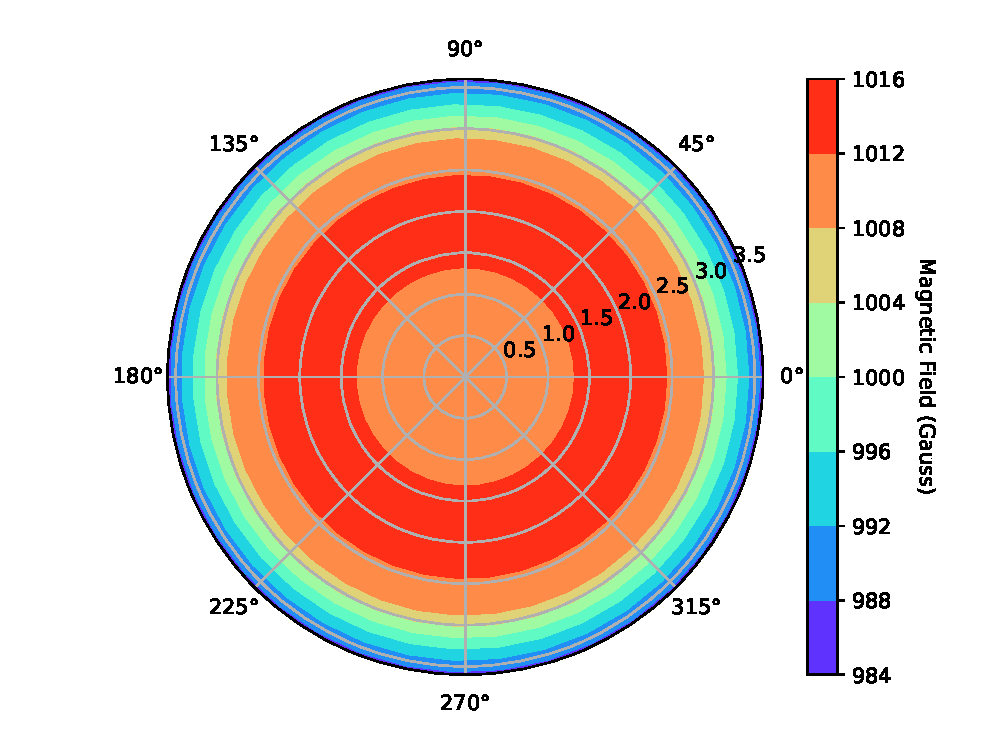
\includegraphics[width=1\columnwidth]{images/contour0.5.eps}
    \caption{Contour Plot of the Magnetic Field Distribution across the circular surface at Coil current $= 0.5$ A}
    \label{g1}
\end{figure}

\begin{figure}
    \centering
    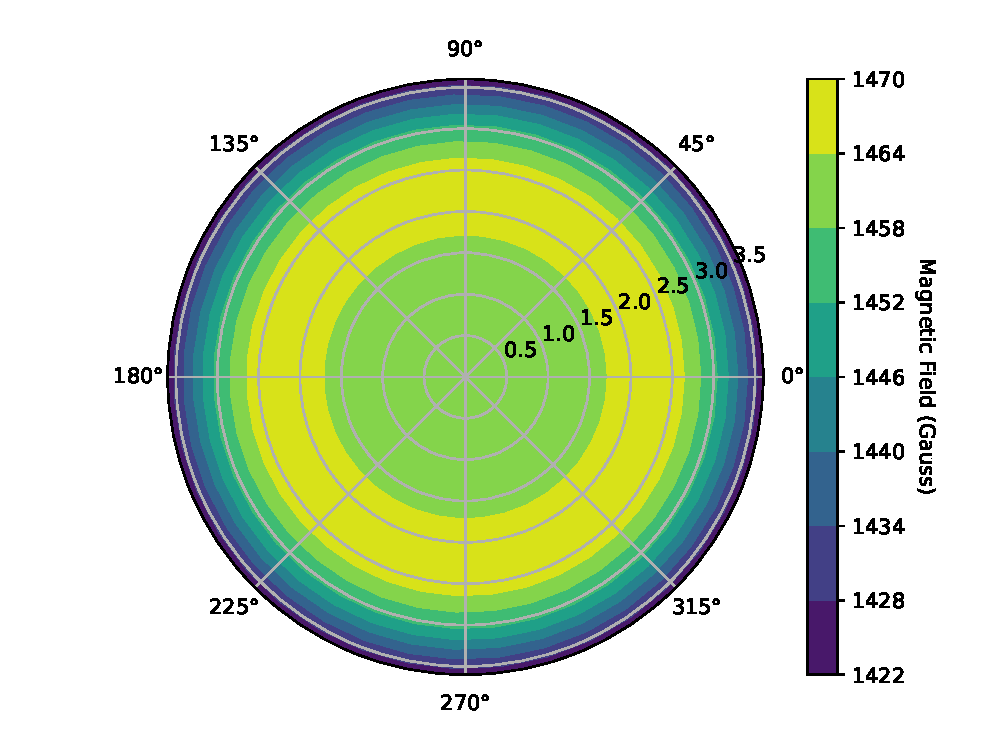
\includegraphics[width=1\columnwidth]{images/contour1.eps}
    \caption{Contour Plot of the Magnetic Field Distribution across the circular surface at Coil current $= 1$ A}
    \label{g2}
\end{figure}

We can see that the variation in the inner region is within 10 Gauss, which is the least count of the Gaussmeter. So any variation would be undetectable with our current measuring setups. Hence we have neglected this deviation in the following sections.

\subsubsection*{Estimation of $R_m$}
Now, after checking that the magnetoresistance setup, preloaded with bismuth, responded to the supplied current, we connect the  outer probe pair connected to the CCS-01 terminals and the inner
pair to the DMV-001 terminals.
We then positioned the magnetoresistance probe and Hall sensor vertically aligned. Using the constant current source, we recorded the magnetic field versus voltage, and determined the resistance ($R_m$) in the presence of the magnetic field for two different sets of probe current. We measured the voltage at zero magnetic field to calculate the resistance ($R$) of the sample. The data
is shown in Tables \ref{trm1} \ref{trm1}.

\begin{table*}[]
    \centering
    \begin{tabular}{|cccccc|cccccc|}
    \hline
        \multicolumn{6}{|c|}{Probe current = 99.5 mA} & \multicolumn{6}{c|}{Probe current = 198.0 mA} \\ \hline
        \multicolumn{1}{|c|}{Magnetic Field} & \multicolumn{1}{c|}{Voltage} & \multicolumn{1}{c|}{$R_m$} & \multicolumn{1}{c|}{$\Delta R$} & \multicolumn{1}{c|}{$\Delta R/R$} & $\log (H)$ & \multicolumn{1}{c|}{Magnetic Field} & \multicolumn{1}{c|}{Voltage} & \multicolumn{1}{c|}{$R_m$} & \multicolumn{1}{c|}{$\Delta R$} & \multicolumn{1}{c|}{$\Delta R/R$} & $\log (H)$ \\
        \multicolumn{1}{|c|}{$H$ (G)} & \multicolumn{1}{c|}{$V_m$ (mV)} & \multicolumn{1}{c|}{($\times 10^{-4}\,\Omega$)} & \multicolumn{1}{c|}{($\times 10^{-4}\,\Omega$)} & \multicolumn{1}{c|}{} &  & \multicolumn{1}{c|}{$H$ (G)} & \multicolumn{1}{c|}{$V_m$ (mV)} & \multicolumn{1}{c|}{($\times 10^{-4}\,\Omega$)} & \multicolumn{1}{c|}{($\times 10^{-4}\,\Omega$)} & \multicolumn{1}{c|}{} &  \\ \hline
       
        \multicolumn{1}{|c|}{0} & \multicolumn{1}{c|}{0.063} & \multicolumn{1}{c|}{6.332} & \multicolumn{1}{c|}{} & \multicolumn{1}{c|}{} &  & \multicolumn{1}{c|}{0} & \multicolumn{1}{c|}{0.146} & \multicolumn{1}{c|}{7.374} & \multicolumn{1}{c|}{} & \multicolumn{1}{c|}{} &  \\ \hline
        \multicolumn{1}{|c|}{86} & \multicolumn{1}{c|}{0.065} & \multicolumn{1}{c|}{6.533} & \multicolumn{1}{c|}{0.201} & \multicolumn{1}{c|}{0.031} & 4.454 & \multicolumn{1}{c|}{96} & \multicolumn{1}{c|}{0.148} & \multicolumn{1}{c|}{7.475} & \multicolumn{1}{c|}{0.101} & \multicolumn{1}{c|}{0.014} & 4.564 \\ \hline
        \multicolumn{1}{|c|}{250} & \multicolumn{1}{c|}{0.064} & \multicolumn{1}{c|}{6.432} & \multicolumn{1}{c|}{0.101} & \multicolumn{1}{c|}{0.016} & 5.521 & \multicolumn{1}{c|}{342} & \multicolumn{1}{c|}{0.149} & \multicolumn{1}{c|}{7.525} & \multicolumn{1}{c|}{0.152} & \multicolumn{1}{c|}{0.020} & 5.835 \\ \hline
        \multicolumn{1}{|c|}{431} & \multicolumn{1}{c|}{0.065} & \multicolumn{1}{c|}{6.533} & \multicolumn{1}{c|}{0.201} & \multicolumn{1}{c|}{0.031} & 6.066 & \multicolumn{1}{c|}{523} & \multicolumn{1}{c|}{0.150} & \multicolumn{1}{c|}{7.576} & \multicolumn{1}{c|}{0.202} & \multicolumn{1}{c|}{0.027} & 6.260 \\ \hline
        \multicolumn{1}{|c|}{602} & \multicolumn{1}{c|}{0.065} & \multicolumn{1}{c|}{6.533} & \multicolumn{1}{c|}{0.201} & \multicolumn{1}{c|}{0.031} & 6.400 & \multicolumn{1}{c|}{712} & \multicolumn{1}{c|}{0.150} & \multicolumn{1}{c|}{7.576} & \multicolumn{1}{c|}{0.202} & \multicolumn{1}{c|}{0.027} & 6.568 \\ \hline
        \multicolumn{1}{|c|}{1088} & \multicolumn{1}{c|}{0.066} & \multicolumn{1}{c|}{6.633} & \multicolumn{1}{c|}{0.302} & \multicolumn{1}{c|}{0.045} & 6.992 & \multicolumn{1}{c|}{1027} & \multicolumn{1}{c|}{0.151} & \multicolumn{1}{c|}{7.626} & \multicolumn{1}{c|}{0.253} & \multicolumn{1}{c|}{0.033} & 6.934 \\ \hline
        \multicolumn{1}{|c|}{1408} & \multicolumn{1}{c|}{0.068} & \multicolumn{1}{c|}{6.834} & \multicolumn{1}{c|}{0.503} & \multicolumn{1}{c|}{0.074} & 7.250 & \multicolumn{1}{c|}{1275} & \multicolumn{1}{c|}{0.153} & \multicolumn{1}{c|}{7.727} & \multicolumn{1}{c|}{0.354} & \multicolumn{1}{c|}{0.046} & 7.151 \\ \hline
        \multicolumn{1}{|c|}{1797} & \multicolumn{1}{c|}{0.068} & \multicolumn{1}{c|}{6.834} & \multicolumn{1}{c|}{0.503} & \multicolumn{1}{c|}{0.074} & 7.494 & \multicolumn{1}{c|}{1576} & \multicolumn{1}{c|}{0.154} & \multicolumn{1}{c|}{7.778} & \multicolumn{1}{c|}{0.404} & \multicolumn{1}{c|}{0.052} & 7.363 \\ \hline
        \multicolumn{1}{|c|}{2580} & \multicolumn{1}{c|}{0.069} & \multicolumn{1}{c|}{6.935} & \multicolumn{1}{c|}{0.603} & \multicolumn{1}{c|}{0.087} & 7.856 & \multicolumn{1}{c|}{1752} & \multicolumn{1}{c|}{0.156} & \multicolumn{1}{c|}{7.879} & \multicolumn{1}{c|}{0.505} & \multicolumn{1}{c|}{0.064} & 7.469 \\ \hline
        \multicolumn{1}{|c|}{2800} & \multicolumn{1}{c|}{0.070} & \multicolumn{1}{c|}{7.035} & \multicolumn{1}{c|}{0.704} & \multicolumn{1}{c|}{0.100} & 7.937 & \multicolumn{1}{c|}{2090} & \multicolumn{1}{c|}{0.155} & \multicolumn{1}{c|}{7.828} & \multicolumn{1}{c|}{0.455} & \multicolumn{1}{c|}{0.058} & 7.645 \\ \hline
        \multicolumn{1}{|c|}{3060} & \multicolumn{1}{c|}{0.071} & \multicolumn{1}{c|}{7.136} & \multicolumn{1}{c|}{0.804} & \multicolumn{1}{c|}{0.113} & 8.026 & \multicolumn{1}{c|}{2610} & \multicolumn{1}{c|}{0.158} & \multicolumn{1}{c|}{7.980} & \multicolumn{1}{c|}{0.606} & \multicolumn{1}{c|}{0.076} & 7.867 \\ \hline
        \multicolumn{1}{|c|}{3210} & \multicolumn{1}{c|}{0.073} & \multicolumn{1}{c|}{7.337} & \multicolumn{1}{c|}{1.005} & \multicolumn{1}{c|}{0.137} & 8.074 & \multicolumn{1}{c|}{3330} & \multicolumn{1}{c|}{0.158} & \multicolumn{1}{c|}{7.980} & \multicolumn{1}{c|}{0.606} & \multicolumn{1}{c|}{0.076} & 8.111 \\ \hline
        \multicolumn{1}{|c|}{3460} & \multicolumn{1}{c|}{0.074} & \multicolumn{1}{c|}{7.437} & \multicolumn{1}{c|}{1.106} & \multicolumn{1}{c|}{0.149} & 8.149 & \multicolumn{1}{c|}{3770} & \multicolumn{1}{c|}{0.159} & \multicolumn{1}{c|}{8.030} & \multicolumn{1}{c|}{0.657} & \multicolumn{1}{c|}{0.082} & 8.235 \\ \hline
        \multicolumn{1}{|c|}{3820} & \multicolumn{1}{c|}{0.074} & \multicolumn{1}{c|}{7.437} & \multicolumn{1}{c|}{1.106} & \multicolumn{1}{c|}{0.149} & 8.248 & \multicolumn{1}{c|}{4020} & \multicolumn{1}{c|}{0.163} & \multicolumn{1}{c|}{8.232} & \multicolumn{1}{c|}{0.859} & \multicolumn{1}{c|}{0.104} & 8.299 \\ \hline
        \multicolumn{1}{|c|}{3990} & \multicolumn{1}{c|}{0.075} & \multicolumn{1}{c|}{7.538} & \multicolumn{1}{c|}{1.206} & \multicolumn{1}{c|}{0.160} & 8.292 & \multicolumn{1}{c|}{4230} & \multicolumn{1}{c|}{0.165} & \multicolumn{1}{c|}{8.333} & \multicolumn{1}{c|}{0.960} & \multicolumn{1}{c|}{0.115} & 8.350 \\ \hline
        \multicolumn{1}{|c|}{4440} & \multicolumn{1}{c|}{0.077} & \multicolumn{1}{c|}{7.739} & \multicolumn{1}{c|}{1.407} & \multicolumn{1}{c|}{0.182} & 8.398 & \multicolumn{1}{c|}{4420} & \multicolumn{1}{c|}{0.167} & \multicolumn{1}{c|}{8.434} & \multicolumn{1}{c|}{1.061} & \multicolumn{1}{c|}{0.126} & 8.394 \\ \hline
        \multicolumn{1}{|c|}{4960} & \multicolumn{1}{c|}{0.078} & \multicolumn{1}{c|}{7.839} & \multicolumn{1}{c|}{1.508} & \multicolumn{1}{c|}{0.192} & 8.509 & \multicolumn{1}{c|}{4780} & \multicolumn{1}{c|}{0.169} & \multicolumn{1}{c|}{8.535} & \multicolumn{1}{c|}{1.162} & \multicolumn{1}{c|}{0.136} & 8.472 \\ \hline
        \multicolumn{1}{|c|}{} & \multicolumn{1}{c|}{} & \multicolumn{1}{c|}{} & \multicolumn{1}{c|}{} & \multicolumn{1}{c|}{} &  & \multicolumn{1}{c|}{5110} & \multicolumn{1}{c|}{0.169} & \multicolumn{1}{c|}{8.535} & \multicolumn{1}{c|}{1.162} & \multicolumn{1}{c|}{0.136} & 8.539 \\ \hline
        \multicolumn{1}{|c|}{} & \multicolumn{1}{c|}{} & \multicolumn{1}{c|}{} & \multicolumn{1}{c|}{} & \multicolumn{1}{c|}{} &  & \multicolumn{1}{c|}{5210} & \multicolumn{1}{c|}{0.170} & \multicolumn{1}{c|}{8.586} & \multicolumn{1}{c|}{1.212} & \multicolumn{1}{c|}{0.141} & 8.558 \\ \hline
        \multicolumn{1}{|c|}{} & \multicolumn{1}{c|}{} & \multicolumn{1}{c|}{} & \multicolumn{1}{c|}{} & \multicolumn{1}{c|}{} &  & \multicolumn{1}{c|}{5420} & \multicolumn{1}{c|}{0.173} & \multicolumn{1}{c|}{8.737} & \multicolumn{1}{c|}{1.364} & \multicolumn{1}{c|}{0.156} & 8.598 \\ \hline
        \end{tabular}
        \caption{Magnetoresistance data for both values of probe currents}
        \label{trm1}
\end{table*}
    % Magnetic Field & Voltage  & $R_m$  & $\Delta R$ & $\Delta R/R$ & $\log (H)$ &  Magnetic Field & Voltage  & $R_m$  & $\Delta R$ & $\Delta R/R$ & $\log (H)$\\ 
    % $H$ (G) &$V_m$ (mV) & ($\times 10^{-4}\,\Omega$) & ($\times 10^{-4}\,\Omega$) & & & $H$ (G) &$V_m$ (mV) & ($\times 10^{-4}\,\Omega$) & ($\times 10^{-4}\,\Omega$) & &  \\ \hline
    % 0 & 0.063 & 6.332 &  &  & 0 & 0.146 & 7.374 &  &  &  &  \\ \hline
    % 86 & 0.065 & 6.533 & 0.201 & 0.031 & 4.454 & 96 & 0.148 & 7.475 & 0.101 & 0.014 & 4.564 \\ \hline
    % 250 & 0.064 & 6.432 & 0.101 & 0.016 & 5.521 & 342 & 0.149 & 7.525 & 0.152 & 0.020 & 5.835 \\ \hline
    % 431 & 0.065 & 6.533 & 0.201 & 0.031 & 6.066 & 523 & 0.150 & 7.576 & 0.202 & 0.027 & 6.260 \\ \hline
    % 602 & 0.065 & 6.533 & 0.201 & 0.031 & 6.400 & 712 & 0.150 & 7.576 & 0.202 & 0.027 & 6.568 \\ \hline
    % 1088 & 0.066 & 6.633 & 0.302 & 0.045 & 6.992 & 1027 & 0.151 & 7.626 & 0.253 & 0.033 & 6.934 \\ \hline
    % 1408 & 0.068 & 6.834 & 0.503 & 0.074 & 7.250 & 1275 & 0.153 & 7.727 & 0.354 & 0.046 & 7.151 \\ \hline
    % 1797 & 0.068 & 6.834 & 0.503 & 0.074 & 7.494 & 1576 & 0.154 & 7.778 & 0.404 & 0.052 & 7.363 \\ \hline
    % 2580 & 0.069 & 6.935 & 0.603 & 0.087 & 7.856 & 1752 & 0.156 & 7.879 & 0.505 & 0.064 & 7.469 \\ \hline
    % 2800 & 0.070 & 7.035 & 0.704 & 0.100 & 7.937 & 2090 & 0.155 & 7.828 & 0.455 & 0.058 & 7.645 \\ \hline
    % 3060 & 0.071 & 7.136 & 0.804 & 0.113 & 8.026 & 2610 & 0.158 & 7.980 & 0.606 & 0.076 & 7.867 \\ \hline
    % 3210 & 0.073 & 7.337 & 1.005 & 0.137 & 8.074 & 3330 & 0.158 & 7.980 & 0.606 & 0.076 & 8.111 \\ \hline
    % 3460 & 0.074 & 7.437 & 1.106 & 0.149 & 8.149 & 3770 & 0.159 & 8.030 & 0.657 & 0.082 & 8.235 \\ \hline
    % 3820 & 0.074 & 7.437 & 1.106 & 0.149 & 8.248 & 4020 & 0.163 & 8.232 & 0.859 & 0.104 & 8.299 \\ \hline
    % 3990 & 0.075 & 7.538 & 1.206 & 0.160 & 8.292 & 4230 & 0.165 & 8.333 & 0.960 & 0.115 & 8.350 \\ \hline
    % 4440 & 0.077 & 7.739 & 1.407 & 0.182 & 8.398 & 4420 & 0.167 & 8.434 & 1.061 & 0.126 & 8.394 \\ \hline
    % 4960 & 0.078 & 7.839 & 1.508 & 0.192 & 8.509 & 4780 & 0.169 & 8.535 & 1.162 & 0.136 & 8.472 \\ \hline
    %  &  &  &  &  &  & 5110 & 0.169 & 8.535 & 1.162 & 0.136 & 8.539 \\ \hline
    %  &  &  &  &  &  & 5210 & 0.170 & 8.586 & 1.212 & 0.141 & 8.558 \\ \hline
    %  &  &  &  &  &  & 5420 & 0.173 & 8.737 & 1.364 & 0.156 & 8.598 \\ \hline


First the probe resistance is calculated for
a finite probe current and voltage in presence of zero
magnetic field. Then this resistance is kept as the
reference for calculating the fractional change in resistance due in applied magnetic field.
Calculations
for magnetoresistance is performed using Eq. \ref{eq8}. Log scale is used in both Fig. \ref{rm1} and Fig. \ref{rm2} to highlight the change in
magnetoresistance across large variation of magnetic
field.

\begin{figure}
    \centering
    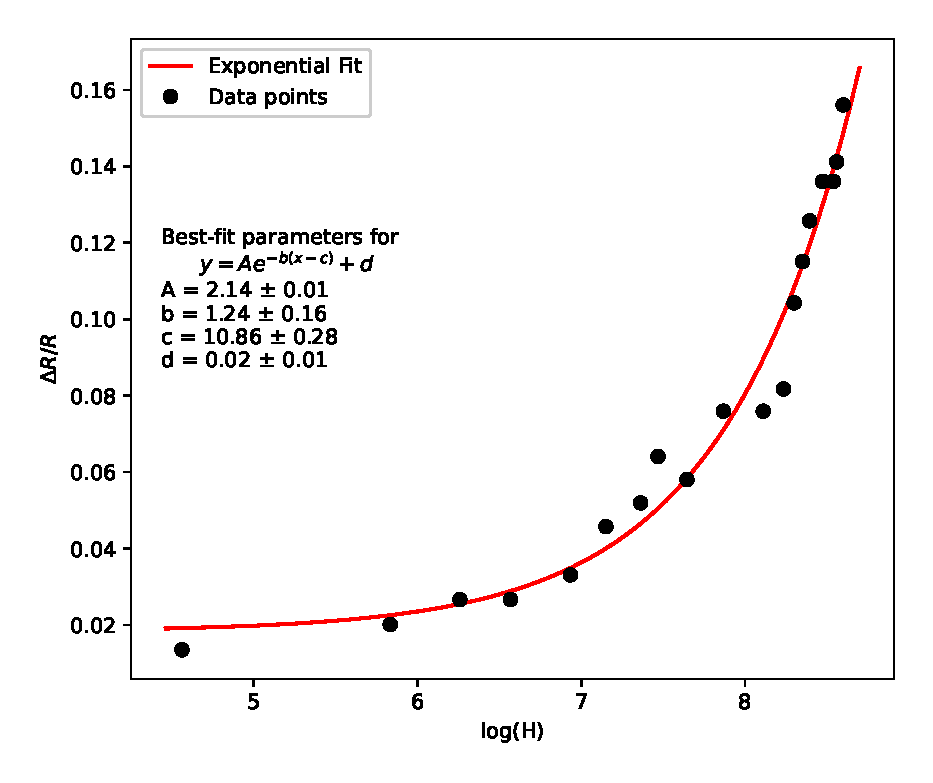
\includegraphics[width=1\columnwidth]{images/198rm.eps}
    \caption{Plot depicting change of resistance w.r.t magnetic field (in log scale) for CCS of 198.0 mA}
    \label{rm1}
\end{figure}
\begin{figure}
    \centering
    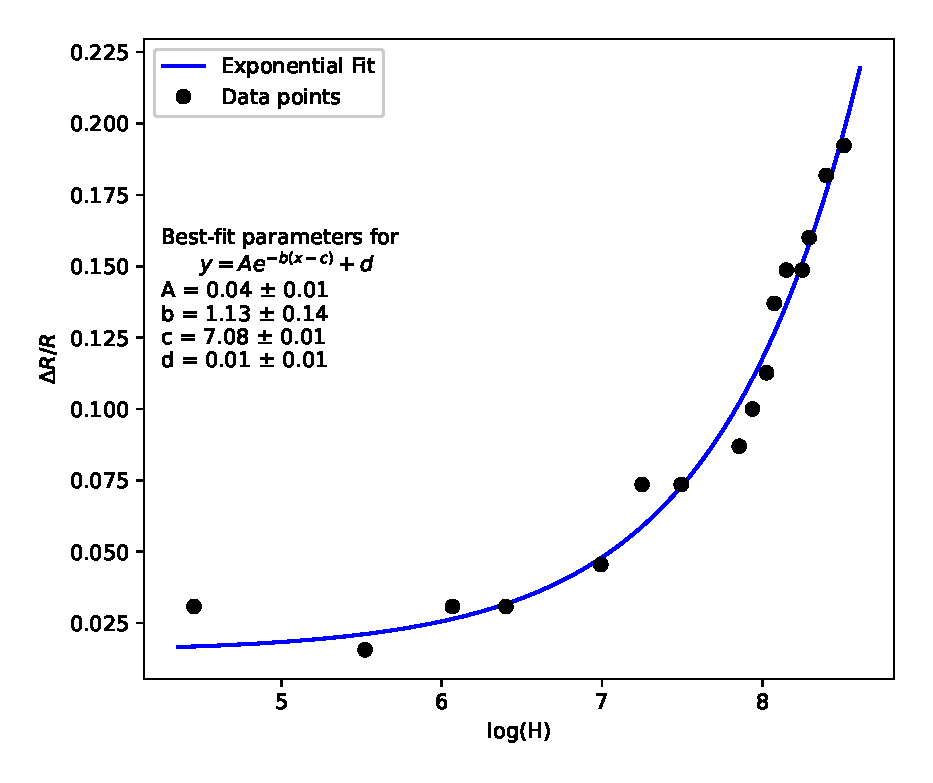
\includegraphics[width=1\columnwidth]{images/99rm.eps}
    \caption{Plot depicting change of resistance w.r.t magnetic field (in log scale) for CCS of 99.5 mA}
    \label{rm2}
\end{figure}

\subsection{Hall Coefficient}

\subsubsection*{Calibration of Magnetic Field vs. Coil Current}
First we calibrated the magnetic field values against the coil current using Table \ref{tab:cal}. 
$H$ was calculated for each $I$ from using $H = (2344.45\cdot I - 396.14)$ Gauss (Fig. \ref{calf}).

\begin{table}[H]
    \centering
    \begin{tabular}{|c|c|c|}
    \hline
    Source & Energy (keV) & Peak Channel \\ \hline
    Ba-133 & 356 & 169.9308 \\ \hline
    Cs-137 & 662 & 302.922 \\ \hline
    Co-60 & 1172 & 525.6078 \\ \hline
    Co-60 & 1335 & 598.9153 \\ \hline
    \end{tabular}
    \caption{Known energy sources calibrated across a range of 1024 channels}
    \label{tab:cal}
    \end{table}
\begin{figure}
    \centering
    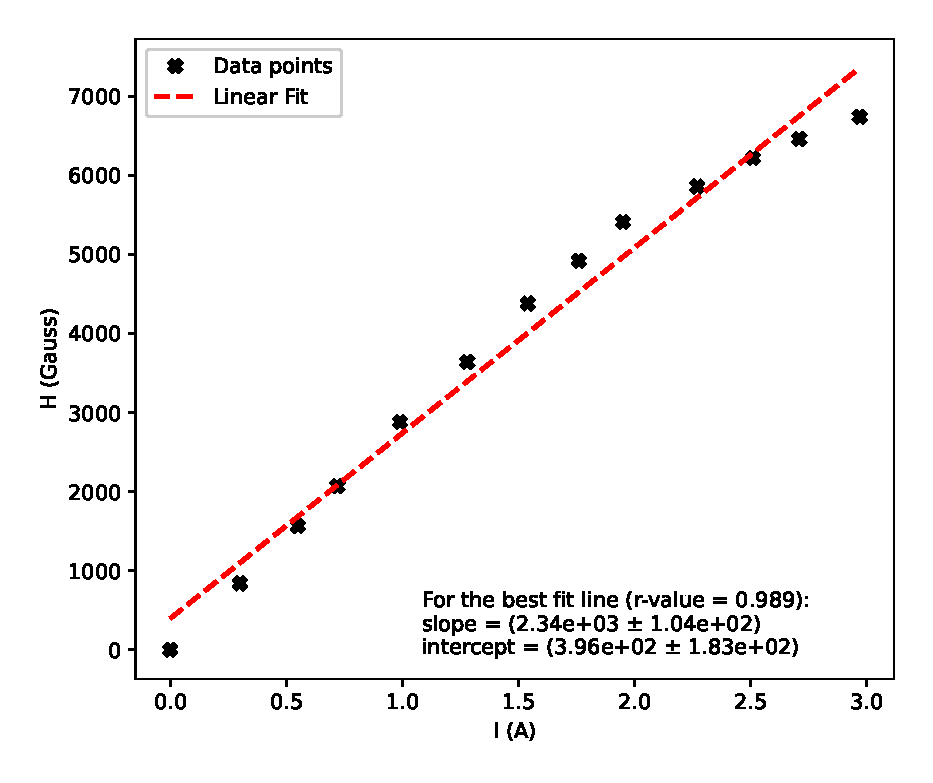
\includegraphics[width=1\columnwidth]{images/cal.eps}
    \caption{Calibration plot of Magnetic field and Coil Current}
    \label{calf}
\end{figure}

\subsubsection*{Estimation of $R_H$}
The Hall voltage against different values of coil currents, for two different values of probe current is shown in Table \ref{tab:coeff}. The Hall voltage as a function of the magnetic field obtained through the calibration curve plot is shown in Figs. \ref{rh1} and \ref{rh2}.
All units have been converted to SI for simplicity.

\begin{table}[]
    \centering
    \begin{tabular}{|cc|cc|}
    \hline
    \multicolumn{2}{|c|}{$I=119.0$ mA} & \multicolumn{2}{c|}{$I=198.2$ mA} \\ \hline
    \multicolumn{1}{|c|}{I (A)} & Hall Voltage (mV) & \multicolumn{1}{c|}{I (A)} & Hall Voltage (mV) \\ \hline
    \multicolumn{1}{|c|}{0.12} & -0.004 & \multicolumn{1}{c|}{0.00} & 0.000 \\ \hline
    \multicolumn{1}{|c|}{0.23} & -0.008 & \multicolumn{1}{c|}{0.15} & -0.004 \\ \hline
    \multicolumn{1}{|c|}{0.40} & -0.014 & \multicolumn{1}{c|}{0.40} & -0.018 \\ \hline
    \multicolumn{1}{|c|}{0.60} & -0.021 & \multicolumn{1}{c|}{0.60} & -0.028 \\ \hline
    \multicolumn{1}{|c|}{0.80} & -0.029 & \multicolumn{1}{c|}{0.82} & -0.042 \\ \hline
    \multicolumn{1}{|c|}{1.02} & -0.036 & \multicolumn{1}{c|}{1.01} & -0.050 \\ \hline
    \multicolumn{1}{|c|}{1.20} & -0.039 & \multicolumn{1}{c|}{1.20} & -0.055 \\ \hline
    \multicolumn{1}{|c|}{1.40} & -0.045 & \multicolumn{1}{c|}{1.42} & -0.066 \\ \hline
    \multicolumn{1}{|c|}{1.53} & -0.048 & \multicolumn{1}{c|}{1.60} & -0.073 \\ \hline
    \multicolumn{1}{|c|}{1.82} & -0.048 & \multicolumn{1}{c|}{1.82} & -0.075 \\ \hline
    \multicolumn{1}{|c|}{1.98} & -0.050 & \multicolumn{1}{c|}{} &  \\ \hline
    \multicolumn{1}{|c|}{2.32} & -0.054 & \multicolumn{1}{c|}{} &  \\ \hline
    \multicolumn{1}{|c|}{2.54} & -0.056 & \multicolumn{1}{c|}{} &  \\ \hline
    \multicolumn{1}{|c|}{2.70} & -0.057 & \multicolumn{1}{c|}{} &  \\ \hline
    \multicolumn{1}{|c|}{2.92} & -0.058 & \multicolumn{1}{c|}{} &  \\ \hline
    \multicolumn{1}{|c|}{3.03} & -0.059 & \multicolumn{1}{c|}{} &  \\ \hline
    \end{tabular}
    \caption{Coil current and Hall voltage data for two different probe currents}
    \label{tab:coeff}
\end{table}
\begin{figure}
    \centering
    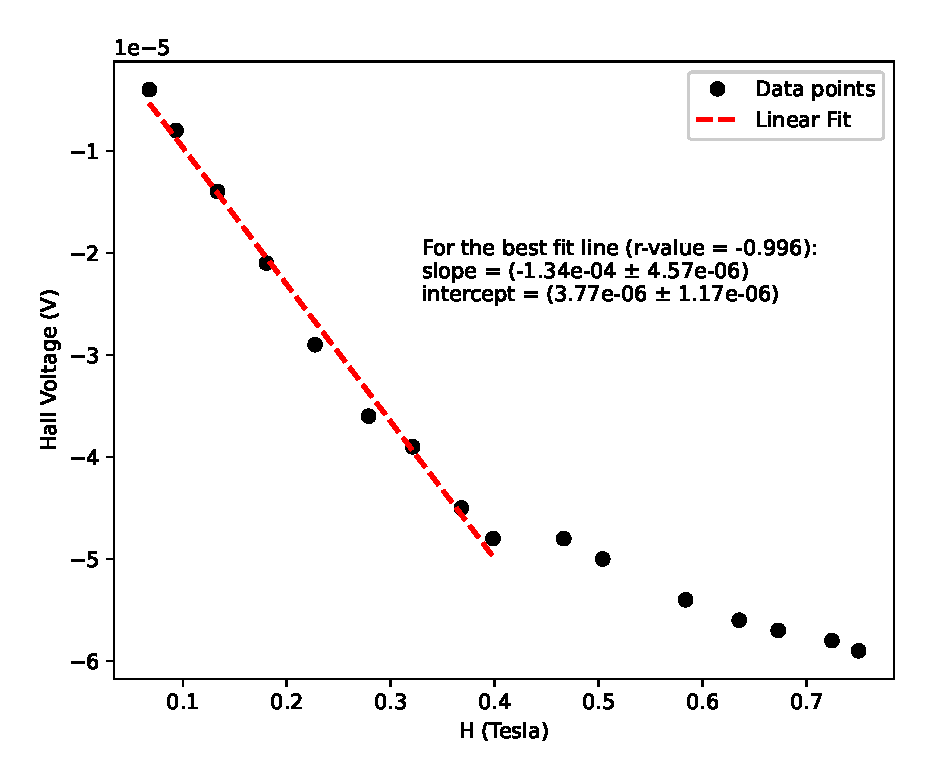
\includegraphics[width=1\columnwidth]{images/119rh.eps}
    \caption{Plot of Hall voltage against applied magnetic field for CCS 119.0 mA}
    \label{rh1}
\end{figure}
\begin{figure}
    \centering
    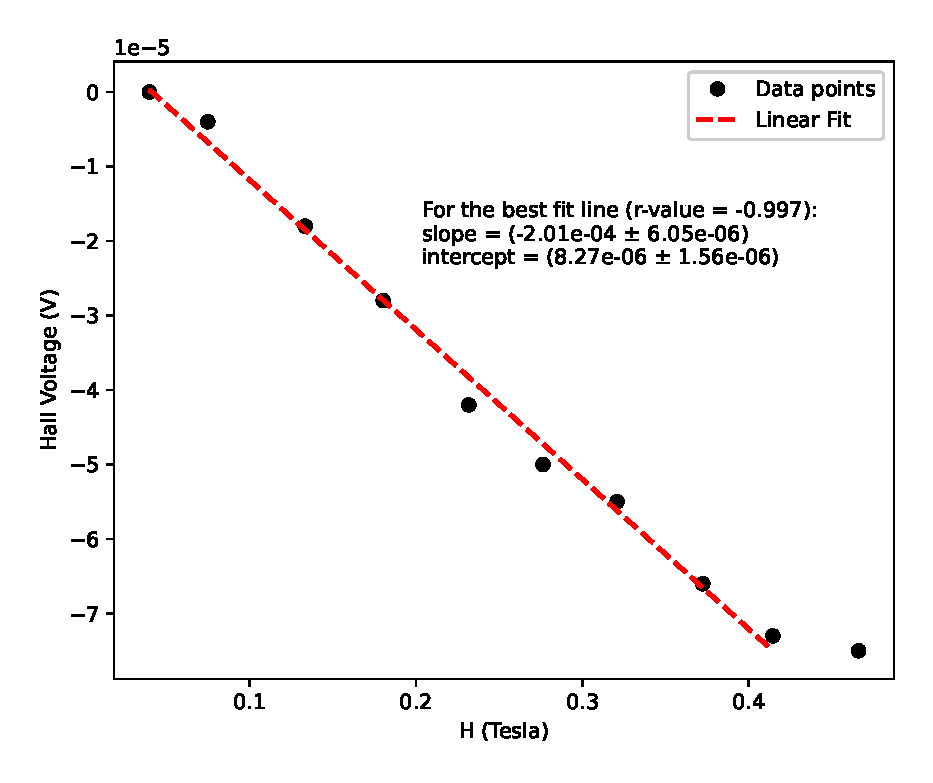
\includegraphics[width=1\columnwidth]{images/198rh.eps}
    \caption{Plot of Hall voltage against applied magnetic field for CCS 198.2 mA}
    \label{rh2}
\end{figure}

We can rewrite Eq. \ref{eq7} as,

\begin{align} \label{eq9}
    R_H = \left(\frac{V}{H}\right)\frac{t}{I}
\end{align}

where the $V/H$ is the slope of the above plot, $I$ refers to the probe current and $t$ is the thickness of the sample which is 0.5mm. Plugging in the values, the Hall coefficient comes out to be:

\begin{itemize}
    \item For $I=119.0$ mA, $R_H = -564.64 $ mm$^3$/C
    \item For $I=198.2$ mA, $R_H = -506.95 $ mm$^3$/C
\end{itemize}

\noindent Since $R_H=1/ne$, we can also derive the charge carrier density to be,

\begin{itemize}
    \item For $I=119.0$ mA, $n = 1.11 \times 10^{16} $ mm$^{-3}$
    \item For $I=198.2$ mA, $n = 1.23 \times 10^{16} $ mm$^{-3}$
\end{itemize}

\noindent Similarly using the given resistivity of the sample $1/\sigma=1.3 \times 10^{-4}\,\Omega$ mm, we can find
the mobility of charge carrier for different values of current using the formula, $\mu_e=\sigma R_H$.

\begin{itemize}
    \item For $I=119.0$ mA, $\mu_e = 7.34 \times 10^{-2} $ mm$^{2}$/Vs
    \item For $I=198.2$ mA, $\mu_e = 6.59 \times 10^{-2} $ mm$^{2}$/Vs
\end{itemize} \vspace{-1em}